\documentclass{beamer}

\usetheme{Copenhagen}
\usepackage[utf8]{inputenc}
\usepackage{graphics}

% Slayt basliklarinda kullanilan font boyutu
\setbeamerfont{frametitle}{size=\normalsize}

\title{BM619 Bilgisayarla Görü}
\author{Nurettin Şenyer}
\date{2011}
\institute[CV]{19/x}

\begin{document}

\frame{\titlepage}

\frame {
	\frametitle {Giriş}

	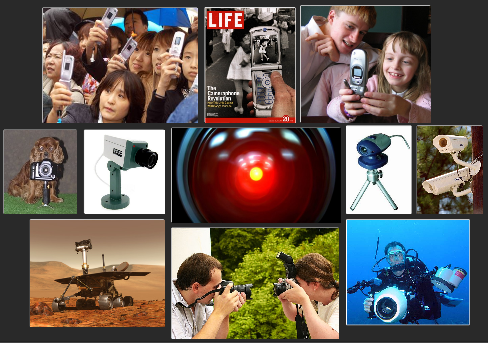
\includegraphics[width=0.9\textwidth]{img/01-giris.png}
}

\frame {
	\frametitle {Bilgisayarla Görünün Amacı}

	Her resmin bir hikayesi vardır,

	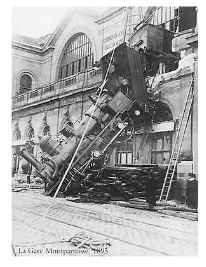
\includegraphics[height=0.9\textheight]{img/01-story}
}

\frame {
	\frametitle {Hikayeyi bilgisayar nasıl görür/anlatır?}

	Resimde olan biteni bilgisayar nasıl söyleyecek?

	\begin{itemize}
		\item Bilgisayarla Görü, piksellerle "anlamı" arasında köprü kurmak
		içindir
	\end{itemize}

	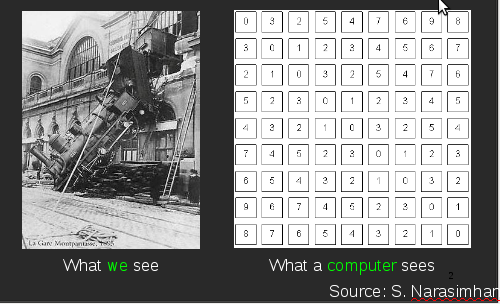
\includegraphics[width=0.9\textwidth]{img/02-amac.png}
}

\frame {
	\frametitle {Bilgisayarla Görü Nedir?}

	\begin{itemize}
		\item anlamı nedir? görmek mi? baktığımız yerdeki şeyi tanımlamak
		\item resimlerden neyi çıkarabiliriz?
		\item :: ne olduğunu?
		\item :: nerede olduğunu?
		\item :: ne yaptığını?
	\end{itemize}
}

\frame {
	\frametitle {Bilgisayarla Görü Nedir?}

	\begin{itemize}[<+->]
		\item Trucco and Verri: bir veya daha fazla resimden 3d dünyanın
		özelliklerini hesaplamak. Örnek: arabanın rengi, hızı
		\medskip
		\item Stockman and Shapiro: algılanan resmi baz alarak gerçek fiziksel
		nesneler ve sahne hakkında faydalı kararlar üretmektir. Örnek: hız limiti aşıldı
		\medskip
		\item Ballard and Brown: resimden fiziksel nesnelerin net, anlamlı
		tanımlar oluşturmaktır. Örnek: arabanın modeli: BMW
		\medskip
		\item Forsyth and Ponce: resimler veya resimler serilerinden dünyaya ait
		tanımlayıcıları çıkartmak. Örnek: arabanın türü: oto
	\end{itemize}
}

\frame {
	\frametitle {Resimden ne tür bilgi çıkarılabilir?}

	\begin{itemize}
		\item \textbf{Metrik} 3d bilgi: derinlik, yükseklik, alan vs

		\medskip

		\item \textbf{Anlamsal} bilgi: ağaç, ev, hareketli, insan vs
	\end{itemize}
}

\frame {
	\frametitle {Metrik: ölçü aleti olarak görü}

	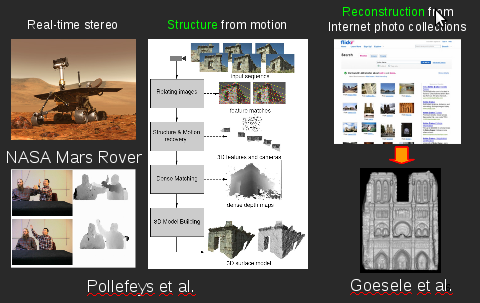
\includegraphics[width=0.9\textwidth]{img/03-metric.png}
}

\frame {
	\frametitle {Anlamsal bilgi kaynağı olarak görü}

	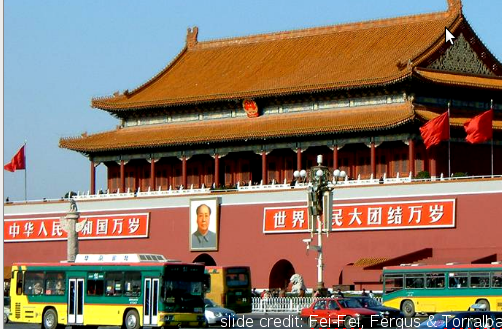
\includegraphics[width=0.9\textwidth]{img/04-semantic.png}
}

\frame {
	\frametitle {Anlamsal: nesne kategorize etme}

	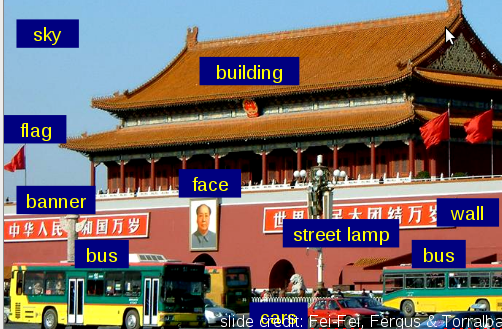
\includegraphics[width=0.9\textwidth]{img/04-semantic2.png}
}

\frame {
	\frametitle {Anlamsal: içerik ve sahne kategorize etme}

	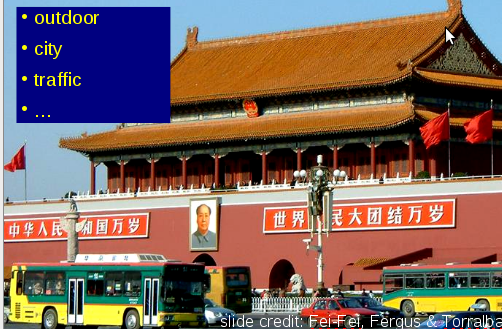
\includegraphics[width=0.9\textwidth]{img/04-semantic3.png}
}

\frame {
	\frametitle {Anlamsal: nitel uzaysal bilgi}

	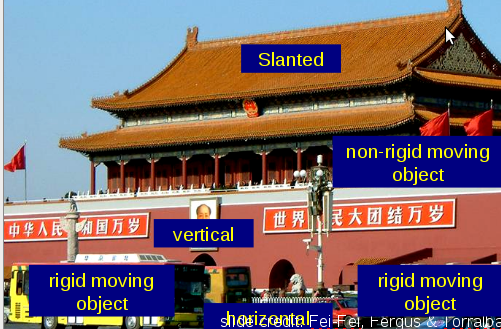
\includegraphics[width=0.9\textwidth]{img/04-semantic4.png}
}

\frame {
	\frametitle {Resimde gördüğünüz nedir?}

	\begin{columns}
		\column{0.5\textwidth}
			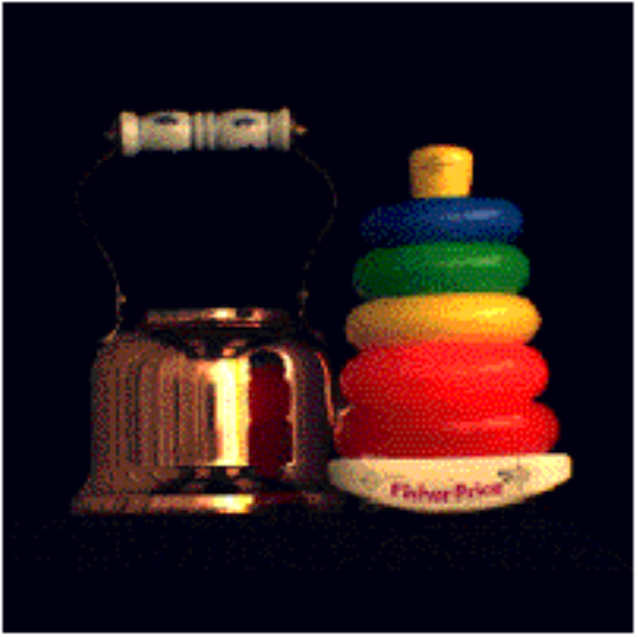
\includegraphics[width=0.9\textwidth]{img/05-mean.png}
			\pause
		\column{0.5\textwidth}
			Siyah arkaplan; iki nesne: çaydanlık, oyuncak; ışık sağdan geliyor;
			birisi parlak diğeri mat; Oyuncak: 5 katlı, farklı renkler, yazı
			var, katmanlar silindir biçimli, plastik, zemin ağaçtan; Çaydanlık:
			gövde ve sap, gövde metalden, sap seramik; sap beyaz üzerinde koyu
			mavi; gövde: altın; gövde üzerine oyuncak yansımış
	\end{columns}
}

\frame {
	\frametitle {Gördüğünüz nedir?}

	\begin{columns}
		\column{0.5\textwidth}
			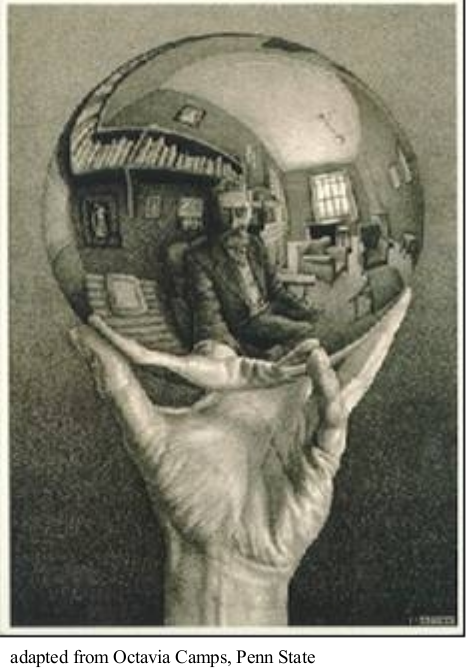
\includegraphics[width=0.9\textwidth]{img/06-what-see.png}
			\pause
		\column{0.5\textwidth}
			\begin{itemize}
				\item adam eli
				\item parlak bir küreyi tutuyor
				\item Escher drawing
			\end{itemize}
	\end{columns}
}

\frame {
	\frametitle {Neden?}

	Görü faydalıdır: resimler ve video heryerde!

	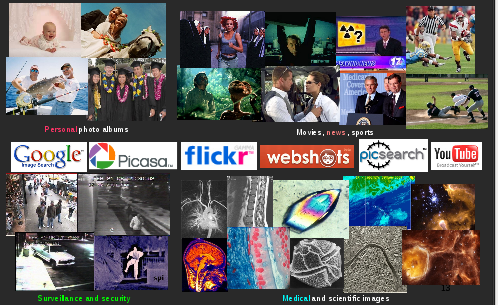
\includegraphics[width=0.95\textwidth]{img/08-why.png}
}

\frame {
	\frametitle {Bilgisayarla Görü Neden Çalışılır?}

	\begin{itemize}
		\item Bir resim 1000 kelimeye bedeldir
		\item resimler ve filmler heryerdedir
		\item hızla gelişen faydalı uygulama koleksiyonu

			\begin{itemize}
				\item resimlerden 3d dünya temsilini oluşturmak
				\item otomatize gözetim (kim ne yapıyor)
				\item film son işleme
				\item yüz bulma
			\end{itemize}

		\item Meydan okuyuş: insan seviyesinde anlayış için daha çok
		çalışmalıyız
	\end{itemize}
}

\frame {
	\frametitle {Bilgisayarla Görü Neden Çalışılır?}

	\begin{itemize}
		\item görü \textbf{faydalıdır}
		\medskip
		\item görü \textbf{ilginçtir}
		\medskip
		\item görü \textbf{zordur}
		\medskip
	\end{itemize}
}

\frame {
	\frametitle {Zorluklar: viewpoint}

	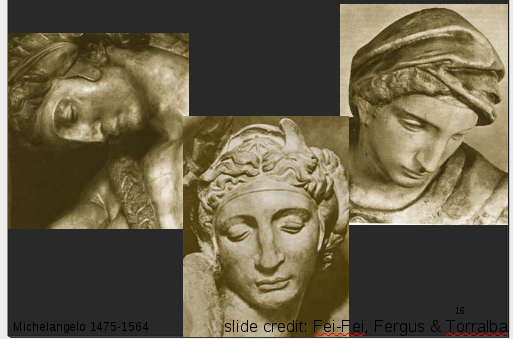
\includegraphics[width=0.9\textwidth]{img/09-viewpoint.png}
}

\frame {
	\frametitle {Zorluklar: illumination}

	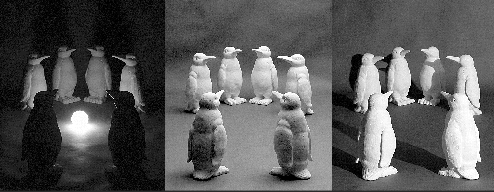
\includegraphics[width=0.9\textwidth]{img/10-illumination.png}
}

\frame {
	\frametitle {Zorluklar: scale}

	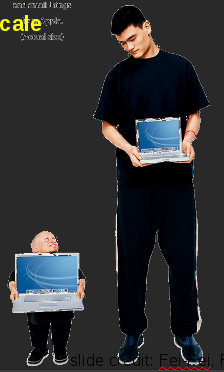
\includegraphics[height=0.9\textheight]{img/11-scale.png}
}

\frame {
	\frametitle {Zorluklar: deform}

	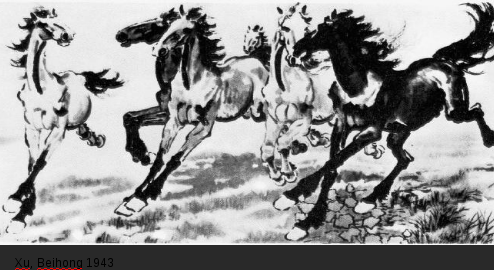
\includegraphics[width=0.9\textwidth]{img/12-deform.png}
}

\frame {
	\frametitle {Zorluklar: perception}

	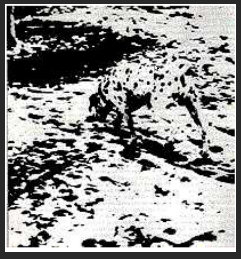
\includegraphics[height=0.9\textheight]{img/13-perception.png}
}

\frame {
	\frametitle {Zorluklar: subject}

	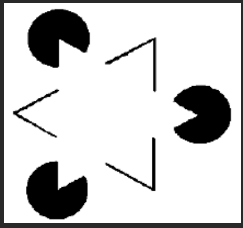
\includegraphics[height=0.9\textheight]{img/14-subject.png}
}

\frame {
	\frametitle {Zorluklar: occlusion}

	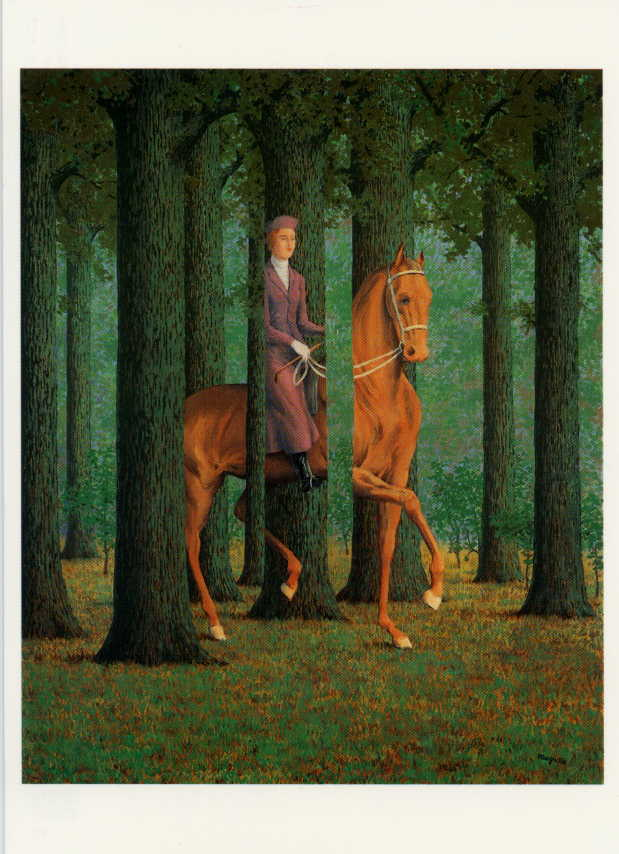
\includegraphics[height=0.9\textheight]{img/15-occlusion.png}
}

\frame {
	\frametitle {Zorluklar: occlusion}

	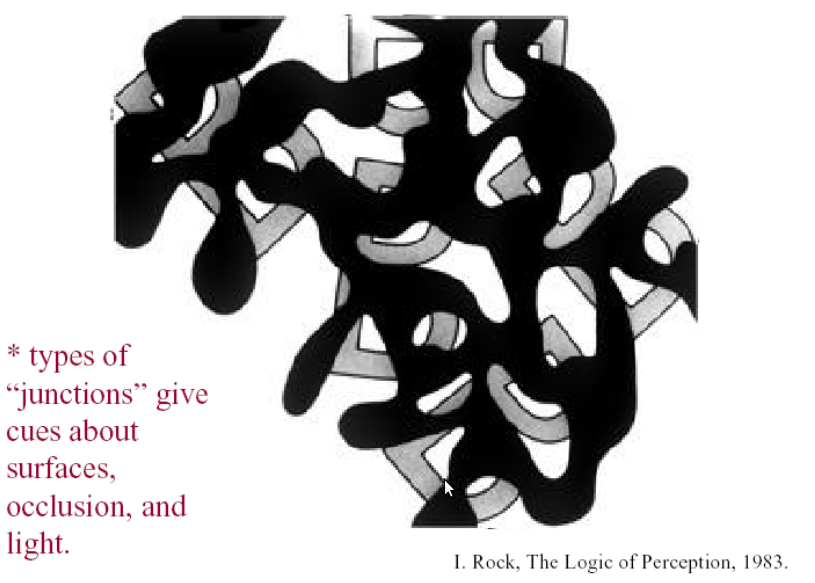
\includegraphics[width=0.9\textwidth]{img/15-occlusion2.png}
}

\frame {
	\frametitle {Zorluklar: junc}

	\begin{columns}
		\column{0.5\textwidth}
			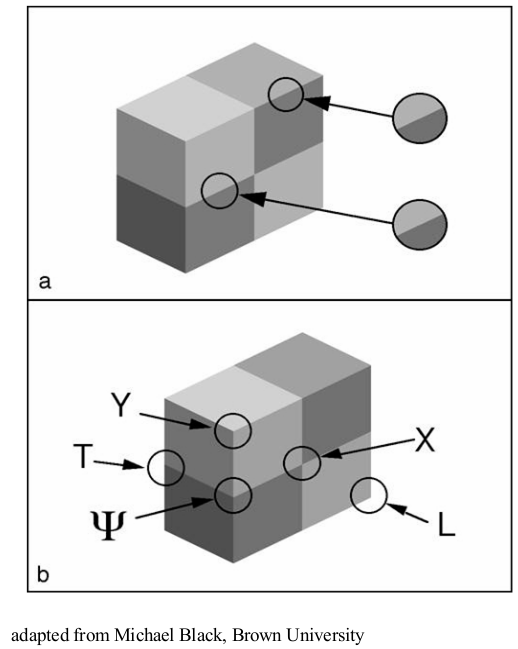
\includegraphics[height=0.9\textheight]{img/16-junc.png}
		\column{0.5\textwidth}
			\begin{itemize}
				\item eklem noktaları sahnenin yorumlanışını kısıtlar
				\item Karışıklık: nesne ve yüzey sınırları birbirine karışabilir
			\end{itemize}
	\end{columns}
}

\frame {
	\frametitle {Zorluklar: clutter}

	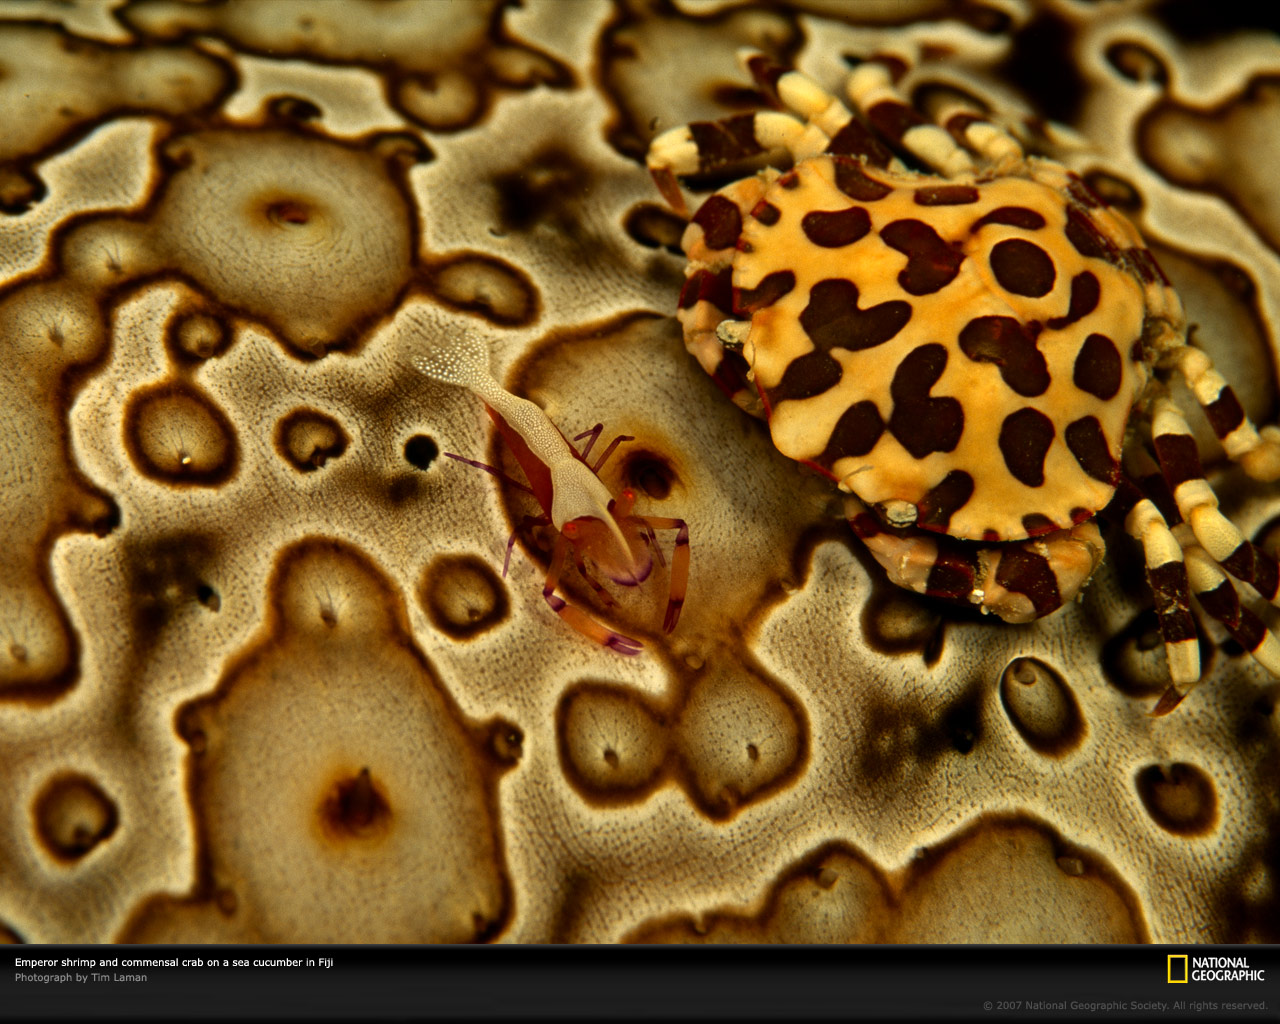
\includegraphics[width=0.9\textwidth]{img/17-clutter.png}
}

\frame {
	\frametitle {Zorluklar: motion}

	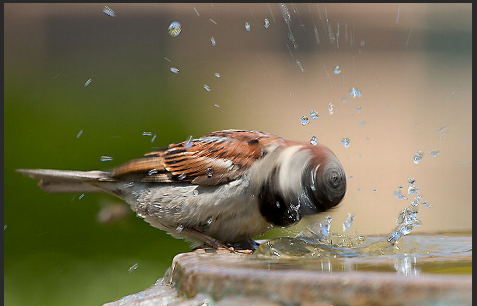
\includegraphics[width=0.9\textwidth]{img/18-motion.png}
}

\frame {
	\frametitle {Zorluklar: variation}

	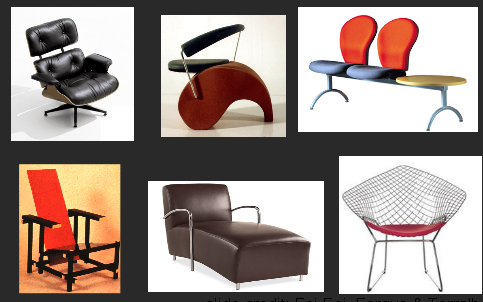
\includegraphics[width=0.9\textwidth]{img/19-variation.png}
}

\frame {
	\frametitle {Zorluklar: ambiguity}

	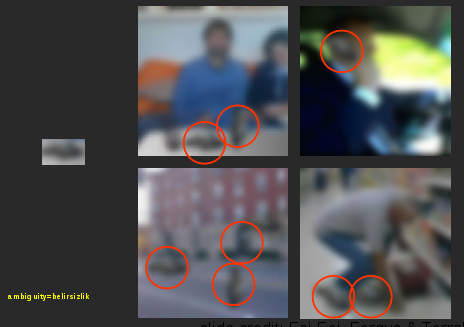
\includegraphics[width=0.9\textwidth]{img/20-ambiguity.png}
}

\frame {
	\frametitle {Zorluklar: dedektif}

	\begin{columns}
		\column{0.5\textwidth}
			\begin{itemize}
				\item Resimler kafa karıştırabilir,
				\item fakat sağladığı ipuçlarıyla dünyayla ilgili bilgi açığa
				vurur
				\item Görevimiz, bu ipuçlarını yorumlamaktır!
			\end{itemize}

		\column{0.5\textwidth}
			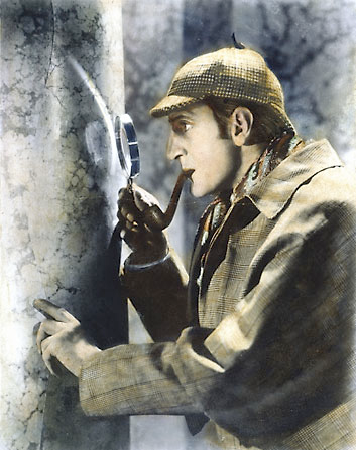
\includegraphics[width=0.9\textwidth]{img/21-dedektif.png}
	\end{columns}
}

\frame {
	\frametitle {İpucu: linear}

	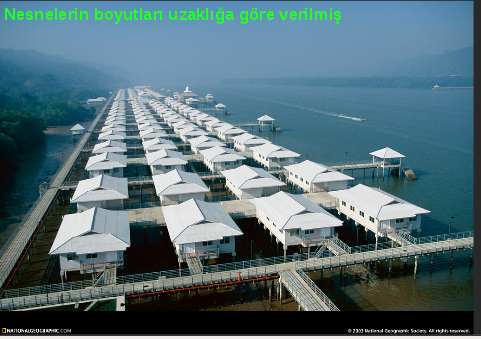
\includegraphics[width=0.9\textwidth]{img/22-linear.png}
}

\frame {
	\frametitle {İpucu: ışık}

	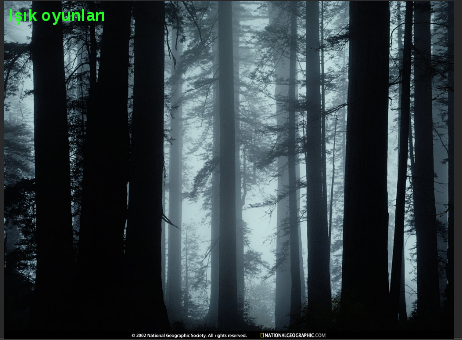
\includegraphics[width=0.9\textwidth]{img/23-isik.png}
}

\frame {
	\frametitle {İpucu: sıra}

	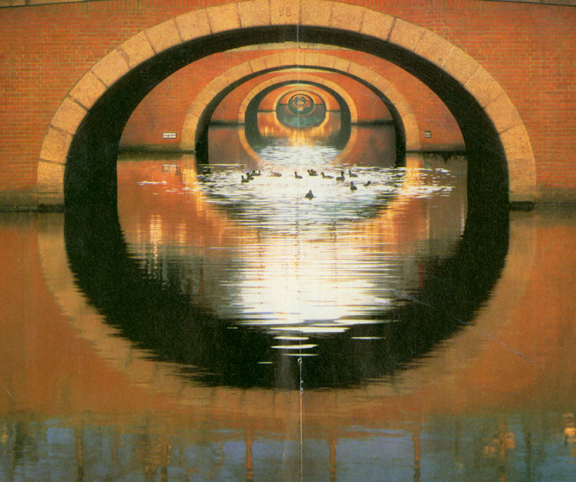
\includegraphics[width=0.9\textwidth]{img/24-order.png}
}

\frame {
	\frametitle {İpucu: texture}

	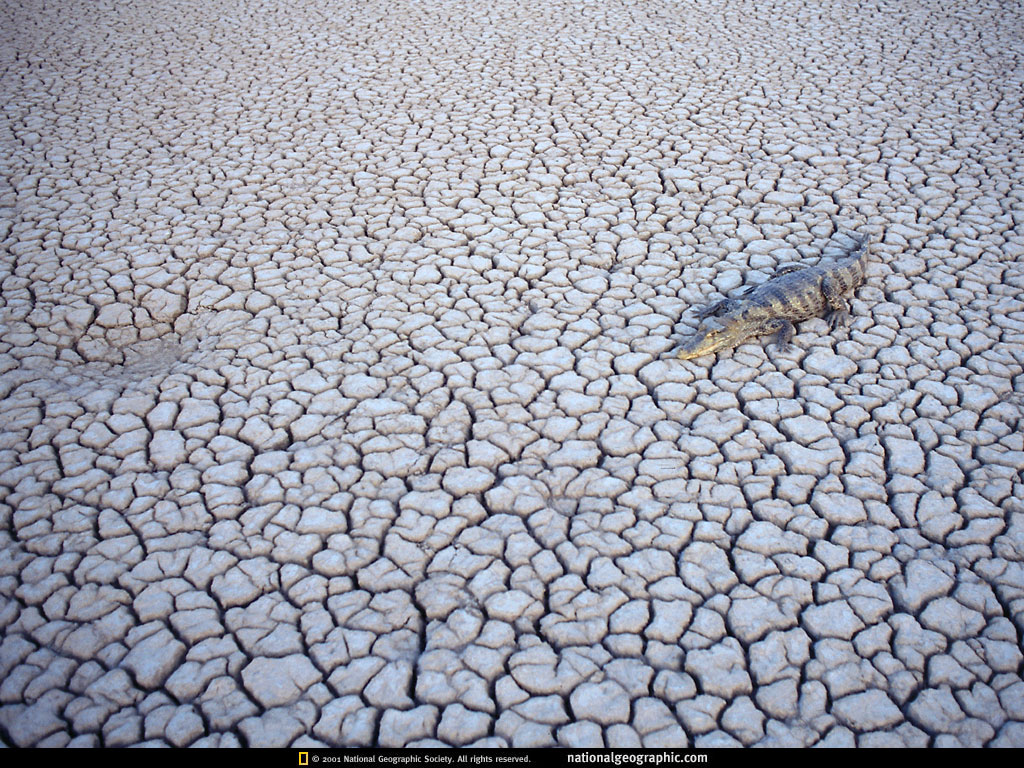
\includegraphics[width=0.9\textwidth]{img/25-texture.png}
}

\frame {
	\frametitle {İpucu: shadow}

	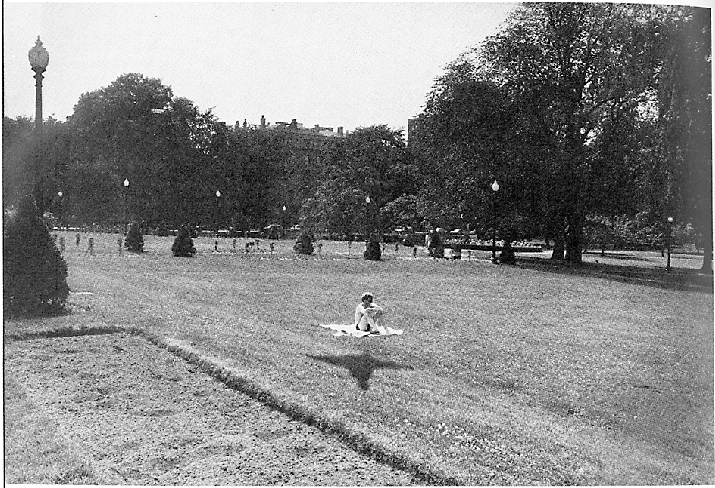
\includegraphics[width=0.9\textwidth]{img/26-shadow.png}
}

\frame {
	\frametitle {İpucu: similarity}

	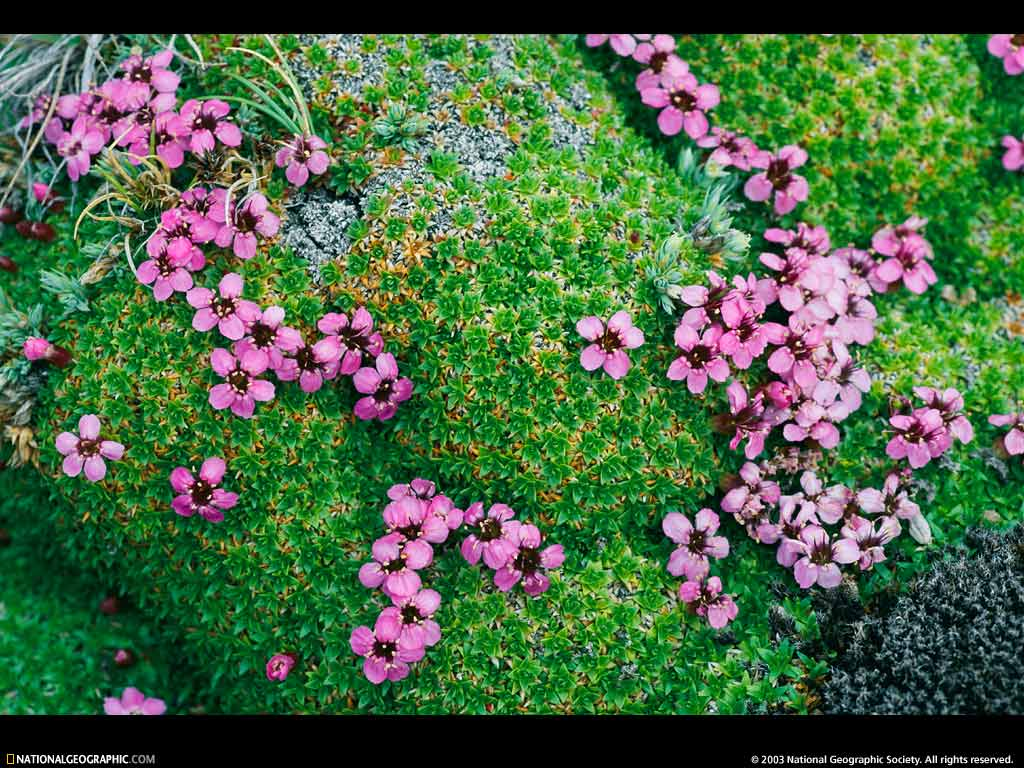
\includegraphics[width=0.9\textwidth]{img/27-similarity.png}
}

\frame {
	\frametitle {İpucu: grup}

	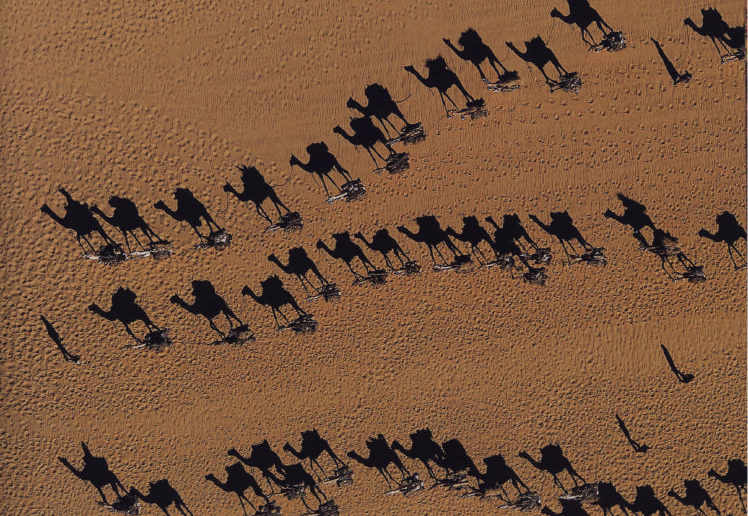
\includegraphics[width=0.9\textwidth]{img/28-grup.png}
}

\frame {
	\frametitle {Sorun: ambiguity}

	\begin{itemize}
		\item Algı, belirsizliği olan bir problemdir
		\item :: Farklı 3d sahneler, aynı 2d resim olarak karşımıza çıkabilir
		\item :: İleri yön: bir sahne $->$ bir resim
		\item :: Geri  yön: bir resim $->$ bir çok sahne

		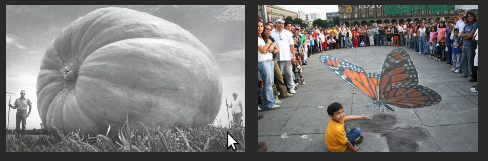
\includegraphics[width=0.9\textwidth]{img/29-ambiguity.png}

		\item Olası çözümler
		\item :: daha fazla kısıtlama (daha fazla resim al)
   		\item :: Yapı hakkında önbilgiyi kullan
		\item Farklı yöntemlerin kombinasyonunu kullan
	\end{itemize}
}

\frame {
	\frametitle {Sorun: algı}

	\begin{itemize}
		\item HVS bazı varsayımlarda bulunur
		\item : Optik ilüzyonlar
	\end{itemize}

	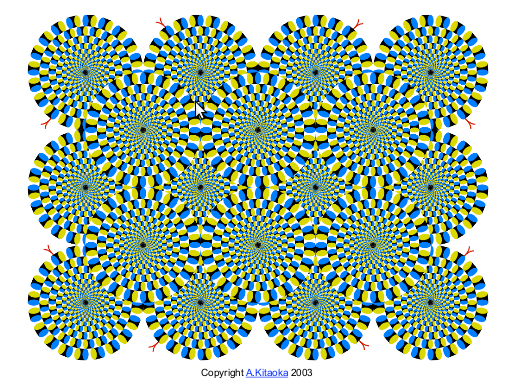
\includegraphics[width=0.9\textwidth]{img/02-algi.png}
}

\frame {
	\frametitle {Disiplin}

	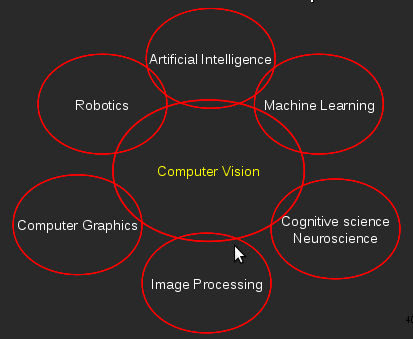
\includegraphics[width=0.9\textwidth]{img/30-disiplin.png}
}

\frame {
	\frametitle {İlişkili Kavramlar}

	\begin{itemize}
		\item Görüntü İşleme:
		\item :: aşağıdaki işleçlerin özelliklerini çalışır
       	\item ::: resimlerden resim üreten
       	\item ::: resimleri filtreleyen ve
       	\item ::: resim işlemeyle ilişkili işleçler
		\item Makine Görü:
   		\item :: şimdilerde Bilgisayarla Görü olarak adlanan terim
   		\item :: endüstriyel görü uygulamaları
   		\item :: tek bir kamerayla yapı hakkında bilgi elde etme
   		\item :: Ters CAD modeli
		\item Örüntü Tanıma:
   		\item :: 2d resimlerdeki yapıları tanımak
       	\item ::: genelde 3d bilgiye referansta bulunmaz
	\end{itemize}
}

\frame {
	\frametitle {İlişkili Kavramlar}

	\begin{itemize}
		\item İşleme
		\item :: Girdi: imge, çıktı: imge
		\item Analiz
   		\item :: Girdi: imge, çıktı: ölçümler
		\item Anlama
   		\item :: Girdi: imge, çıktı: tanımlama
	\end{itemize}
}

\frame {
	\frametitle {Tarihçe}

	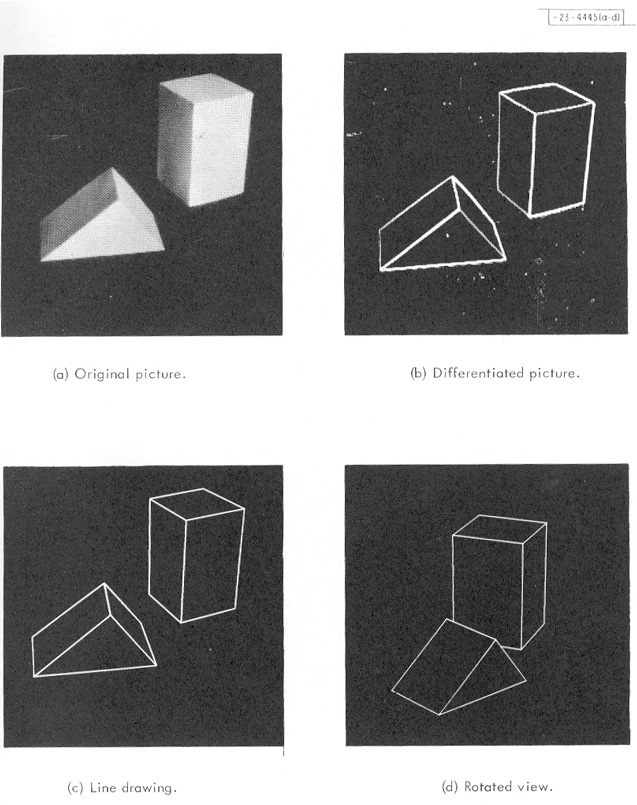
\includegraphics[height=0.9\textheight]{img/31-tarihce.png}

	L. G. Roberts, Machine Perception of Three Dimensional Solids, Ph.D.  thesis,
	MIT Department of Electrical Engineering, 1963.
}

\frame {
	\frametitle {Computer Vision vs. Graphics}

	Görü, Grafiklerin tersi midir?

	\begin{itemize}
		\item Bilgisayar Grafikleri
	    \item :: Resimleri üretir
		\item :: Modeli, koşulları ve görüntüleme parametrelerini seçersiniz
		\item Bilgisayarla Görü
		\item :: Gerçek resimler: gürültülü, örnekleme artifaktlı, ...
		\item :: Fiziksel nitelikleri tahmin et
		\item :: Problemlidir - ihtiyacımız olan minimum bilgi nedir? bilinmez
	\end{itemize}
}

\frame {
	\frametitle {efekt}

	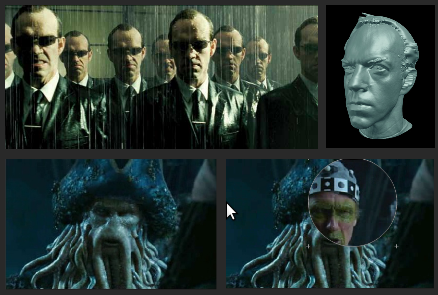
\includegraphics[width=0.9\textwidth]{img/32-efect.png}
}

\frame {
	\frametitle {3d}

	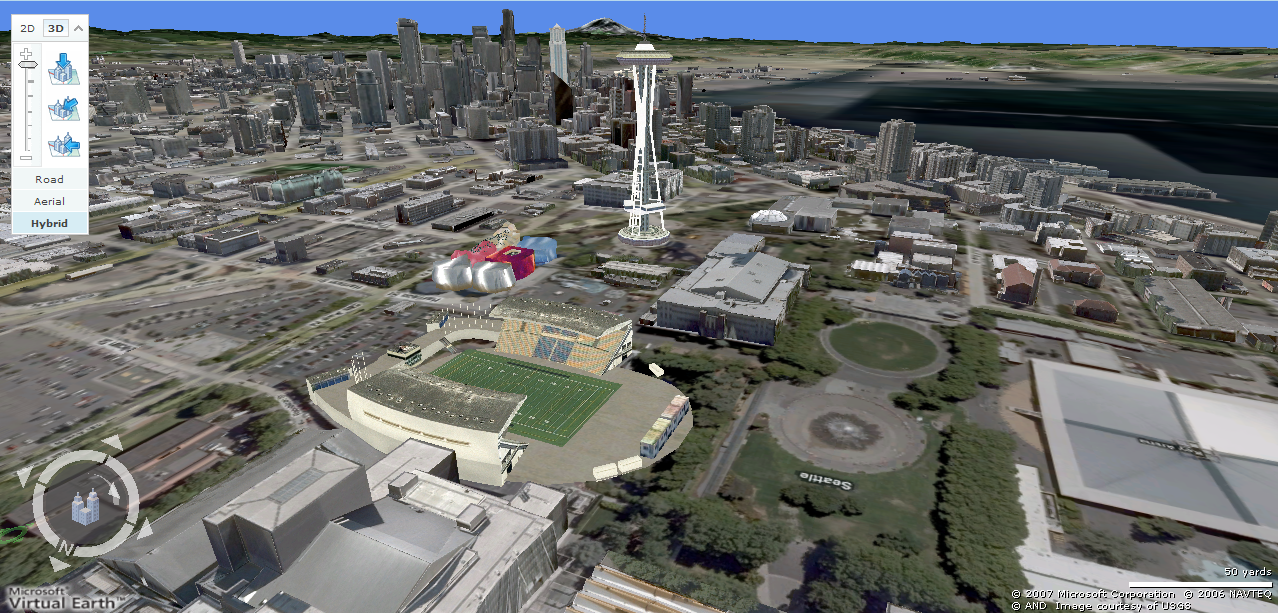
\includegraphics[width=0.9\textwidth]{img/33-3d.png}
}

\frame {
	\frametitle {synth}

	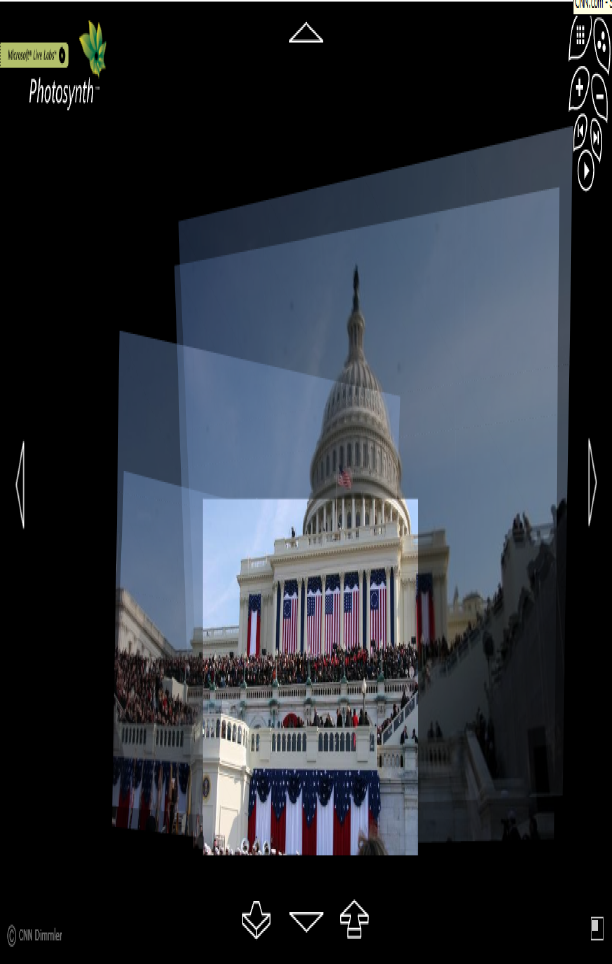
\includegraphics[height=0.7\textheight]{img/34-synt.png}
}

\frame {
	\frametitle {facedet}

	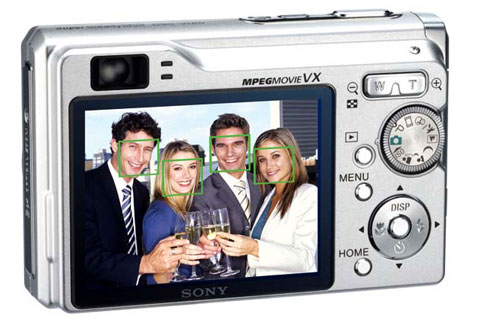
\includegraphics[width=0.9\textwidth]{img/35-facedet.png}
}

\frame {
	\frametitle {smile}

	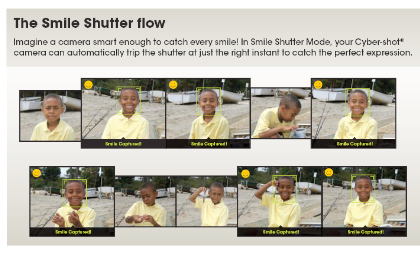
\includegraphics[width=0.9\textwidth]{img/36-smile.png}
}

\frame {
	\frametitle {facerec}

	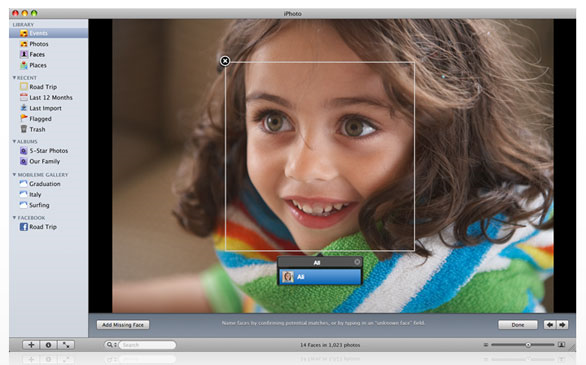
\includegraphics[width=0.9\textwidth]{img/37-facerec.png}
}

\frame {
	\frametitle {facerec}

	\begin{columns}
		\column{0.5\textwidth}
			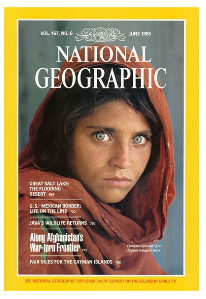
\includegraphics[width=0.9\textwidth]{img/38-afgan.png}
		\column{0.5\textwidth}
			\begin{itemize}
				\item Sharbat Gula at age 12 in an Afgan refugee camp in 1984 Traced
				in 2002 but is she the same person?
			\end{itemize}
	\end{columns}

	Bu kimdir? 2002'de çekilen resimdeki 1984'de çekilen afgan kızı mı?
}

\frame {
	\frametitle {biometrik}

	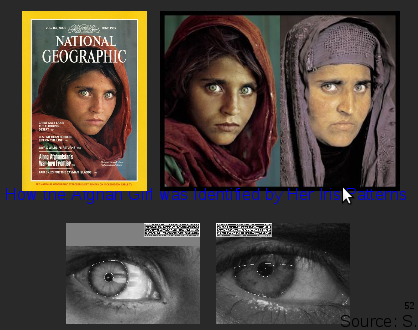
\includegraphics[width=0.9\textwidth]{img/38-bio.png}
}

\frame {
	\frametitle {biometrik}

	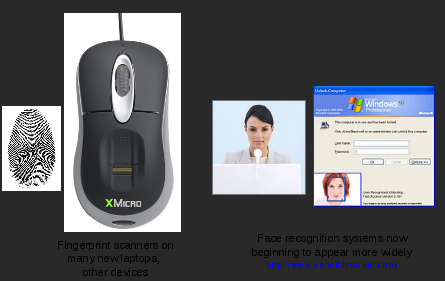
\includegraphics[width=0.9\textwidth]{img/38-biometric2.png}
}

\frame {
	\frametitle {ocr}

	\begin{itemize}
		\item Taranan resmi metne çevirmek
	\end{itemize}

	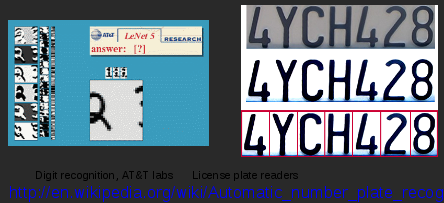
\includegraphics[width=0.9\textwidth]{img/39-ocr.png}
}

\frame {
	\frametitle {goggles}

	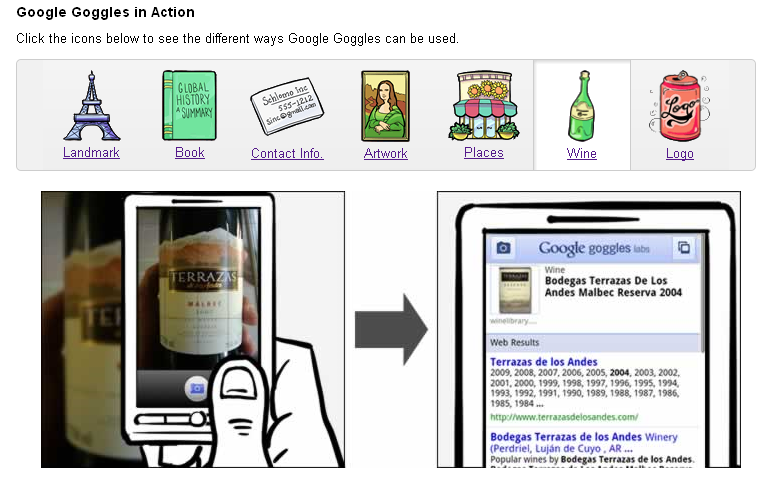
\includegraphics[width=0.9\textwidth]{img/40-goggles.png}
}

\frame {
	\frametitle {phototourism}

	Internet fotograf koleksiyonundan otomatik olarak 3d kurgu.

	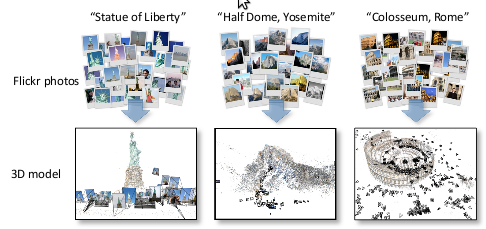
\includegraphics[width=0.9\textwidth]{img/40-phototourism.png}
}

\frame {
	\frametitle {search}

	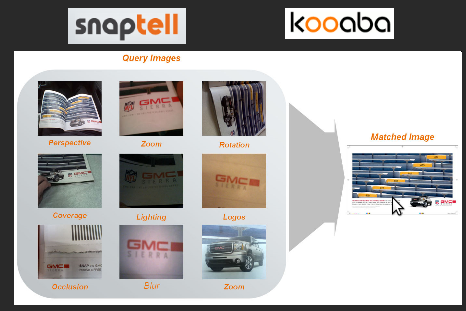
\includegraphics[width=0.9\textwidth]{img/41-search.png}
}

\frame {
	\frametitle {oto}

	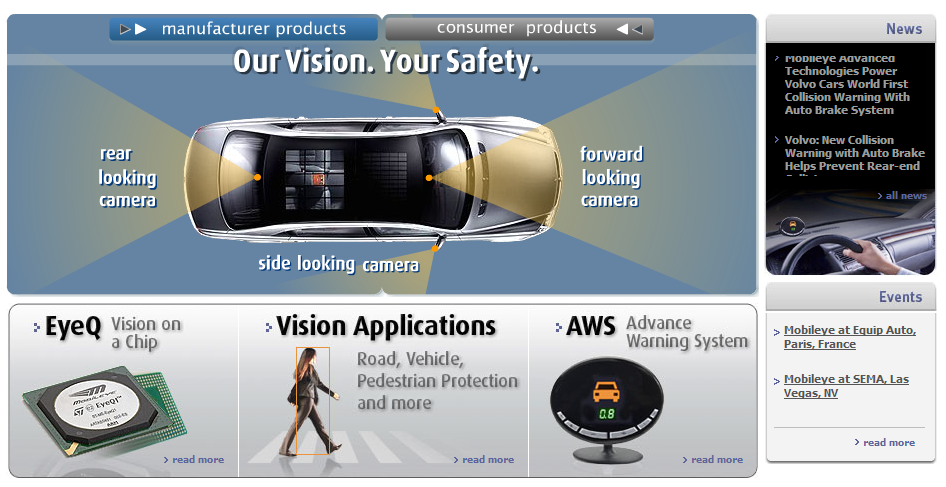
\includegraphics[width=0.9\textwidth]{img/42-oto.png}
}

\frame {
	\frametitle {game}

	\includegraphics[width=0.9\textwidth]{img/43-game.png}
}

\frame {
	\frametitle {market}

	\includegraphics[width=0.9\textwidth]{img/43-market.png}

	LaneHawk by EvolutionRobotics "A smart camera is flush-mounted in the
	checkout lane, continuously watching for items. When an item is detected and
	recognized, the cashier verifies the quantity of items that were found under
	the basket, and continues to close the transaction. The item can remain
	under the basket, and with LaneHawk,you are assured to get paid for it... "
}

\frame {
	\frametitle {robot}

	\includegraphics[width=0.9\textwidth]{img/44-robot.png}

	Vision systems (JPL) used for several tasks
	\begin{itemize}
		\item Panorama stitching
	    \item 3D terrain modeling
		\item Obstacle detection, position tracking
		\item For more, read “Computer Vision on Mars” by Matthies et al.
	\end{itemize}
}

\frame {
	\frametitle {spor}

	\includegraphics[width=0.9\textwidth]{img/41-sport.png}

	Sportvision first down line Nice explanation on www.howstuffworks.com
}

\frame {
	\frametitle {medical}

	\includegraphics[width=0.9\textwidth]{img/42-medical.png}
}

\frame {
	\frametitle {Tanıma: bilgisayarın insan gibi davranması}

	"düşük-seviyeli" metriklerin bir araya gelerek bize neyi söylediğini algısal
	anlamda organize edecek araç $->$ tanıma.

	\medskip

	Çok sayıda ipucu var

	\begin{itemize}
		\item çoklu görüş (hareket, stereo)
		\item doku, doğrusallık, gölge, benzerlik, ...
	\end{itemize}

	\medskip

	Detektif olacaksınız.
}

\frame {
	\frametitle {Tanımada karşılaşılan güçlükler?}

	\begin{itemize}
		\item Hangi bitler birlikte değerlendirilmeli? \pause
		\item :: \textbf{bölütleme} (segmentation)
		\item Ayrıntılarına odaklanmaksızın nesneler nasıl tanınabilir? \pause
		\item :: \textbf{soyutlama} (Abstraction)
		\item Çok sayıda serbestlik derecesi olan nesneler nasıl tanınabilir? \pause
		\item :: popüler bir ismi \textbf{yok}, fakat hayati bir problemdir.
	\end{itemize}
}

\frame {
	\frametitle {Tanıma}

	\includegraphics[width=0.9\textwidth]{img/p01.png}
}

\frame {
	\frametitle {Tanıma}

	\includegraphics[width=0.9\textwidth]{img/p02.png}
}

\frame {
	\frametitle {Tanıma}

	\includegraphics[width=0.9\textwidth]{img/p03.png}
}

\frame {
	\frametitle {Tanıma}

	\includegraphics[width=0.9\textwidth]{img/p04.png}
}

\frame {
	\frametitle {Tanıma}

	\includegraphics[width=0.9\textwidth]{img/p05.png}
}

\frame {
	\frametitle {Tanıma}

	\includegraphics[width=0.75\textwidth]{img/p06.png}

	Muhtemel yaklaşım: çizgi çizmek tanımamızı kolaylaştıracaksa, önce çizgileri
	bulmak
}

\frame {
	\frametitle {Tanıma}

	Çizgi çizmek mi?

	\includegraphics[width=0.9\textwidth]{img/p07.png}
}

\frame {
	\frametitle {Tanıma}

	yoksa kenar algılamak mı?

	\includegraphics[width=0.9\textwidth]{img/p08.png}
}

\frame {
	\frametitle {Tanıma}

	Kenar algılama - parametreleri

	\includegraphics[width=0.9\textwidth]{img/p09.png}
}

\frame {
	\frametitle {Tanıma}

	\includegraphics[width=0.9\textwidth]{img/p10.png}
}

\frame {
	\frametitle {Tanıma}

	\includegraphics[width=0.9\textwidth]{img/p11.png}
}

\frame {
	\frametitle {Tanıma}

	\includegraphics[width=0.9\textwidth]{img/p12.png}
}

\frame {
	\frametitle {Şablon Eşleme}


	\begin{itemize}
		\item bazı nesneler 2d örüntüye sahiptir
		\item :: ör. yüzler
		\medskip

		\item belli bir örüntü eşleyiciyi inşa etmek
		\item :: parametrik modeli kullanarak ışıklanmadaki değişimleri
		indirgemeli
		\item :: arkaplandaki değişimler - zor
		\item :: kamera konumundaki değişimler - zor
	\end{itemize}
}

\frame {
	\frametitle {Tanıma}

	\includegraphics[width=0.9\textwidth]{img/p13.png}
}

\frame {
	\frametitle {Tanıma}

	\includegraphics[width=0.9\textwidth]{img/p14.png}
}

\frame {
	\frametitle {Tanıma}

	yüzü bulmak için farklı yaklaşım:

	\begin{itemize}
		\item önce göz, burun, ağız bul
		\item sonra bu üç bileşen doğru yerleşmiş mi?
	\end{itemize}

	\includegraphics[width=0.9\textwidth]{img/p15.png}
}

\frame {
	\frametitle {Tanıma}

	\begin{columns}
		\column{0.5\textwidth}
		\includegraphics[height=0.9\textheight]{img/p16.png}

		\column{0.5\textwidth}
		Parçaların konumsal ilişkileri ne kadar esnek?
	\end{columns}
}
\frame {
	\frametitle {Tanıma}

	\includegraphics[width=0.9\textwidth]{img/p17.png}
	Bu resimdeki terslik nedir?
}
\frame {
	\frametitle {Tanıma}

	\includegraphics[width=0.9\textwidth]{img/p18.png}
}
\frame {
	\frametitle {Tanıma}

	\begin{columns}
		\column{0.5\textwidth}
			Modeliniz nedir?
			\medskip
			Ne kadar iyi?

		\column{0.5\textwidth}
			\includegraphics[width=0.9\textwidth]{img/p19.png}
	\end{columns}
}
\frame {
	\frametitle {Tanıma}

	\includegraphics[width=0.9\textwidth]{img/p20.png}
}
\frame {
	\frametitle {Tanıma}

	\includegraphics[width=0.9\textwidth]{img/p21.png}
}
\frame {
	\frametitle {Tanıma}

	\includegraphics[width=0.9\textwidth]{img/p22.png}
	Kişi olabilir mi? \pause
	İki slayttaki blob aynı, fakat 90 derece dönmüş
}
\frame {
	\frametitle {Tanıma}

	\includegraphics[width=0.9\textwidth]{img/p23.png}
}
\frame {
	\frametitle {early}

	\includegraphics[width=0.9\textwidth]{img/45-early.png}
}

\frame {
	\frametitle {mid}

	\includegraphics[width=0.9\textwidth]{img/46-mid.png}
}

\frame {
	\frametitle {multi}

	\includegraphics[width=0.9\textwidth]{img/47-multi.png}
}

\frame {
	\frametitle {rec}

	\includegraphics[width=0.9\textwidth]{img/48-rec.png}
}

\frame {
	\frametitle {advanced}

	\includegraphics[width=0.9\textwidth]{img/49-advanced.png}
}

\frame {
	\frametitle {kitap}

	Richard Szeliski, "Computer Vision: Algorithms and Application", Springer, 2010

	\includegraphics[width=0.2\textwidth]{img/50-kitap.png}

	Forsyth and Ponce, Computer Vision: A Modern Approach Richard Szeliski,
	Computer Vision: Algorithms and Applications (draft available online)
}

\end{document}
